% generated by scripts/pkl_to_latex.py
% source PKL : uscan_v1_L8_Ne6_t1_mode-uniform_nmin2_solver-gcg_sz0_restarts10_iter300_kmax4_tol1em09_U1to20_N20-d03a74da789e.pkl
% scan type  : uscan
% state      : gs
% quantity   : linear-entropy
% requires   : \usepackage{pgfplots} \pgfplotsset{compat=1.18}
% colours match the matplotlib PDF (tab10 cycle)
\definecolor{gmeC0}{HTML}{1F77B4}
\definecolor{gmeC1}{HTML}{FF7F0E}
\definecolor{gmeC2}{HTML}{2CA02C}
\definecolor{gmeC3}{HTML}{D62728}
\definecolor{gmeC4}{HTML}{9467BD}
\definecolor{gmeC5}{HTML}{8C564B}
\definecolor{gmeC6}{HTML}{E377C2}
\definecolor{gmeC7}{HTML}{17BECF}

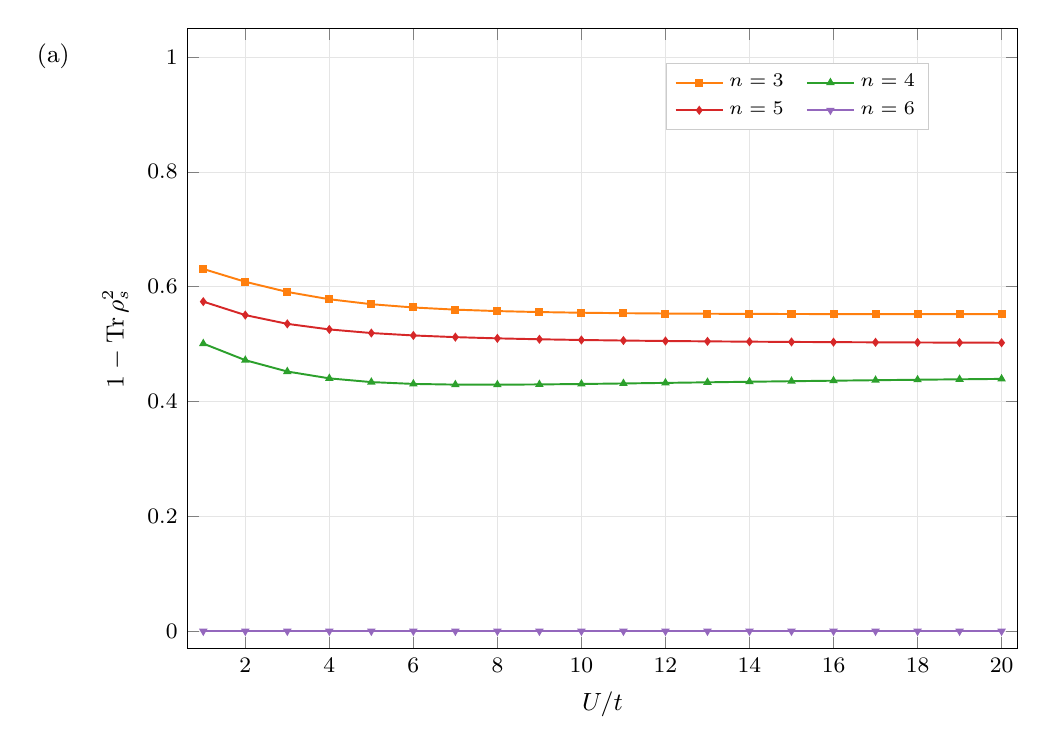
\begin{tikzpicture}
  \begin{axis}[
    width=\columnwidth,
    height=0.78\columnwidth,
    xlabel={$U/t$},
    ylabel={$1-\mathrm{Tr}\,\rho_s^2$},
    grid=both,
    grid style={line width=.1pt, draw=gray!20},
    tick label style={font=\footnotesize\rmfamily, /pgf/number format/fixed},
    label style={font=\small\rmfamily},
    scaled ticks=false,
    legend style={font=\scriptsize\rmfamily, draw=gray!40, at={(0.5,1.03)}, anchor=south, /tikz/every even column/.append style={column sep=6pt}},
    legend cell align={left},
    legend columns=2,
    ymin=-0.03,
    ymax=1.05,
    xmin=0.62,
    xmax=20.38,
    legend style={at={(0.735,0.890)}, anchor=center, fill=white},
    after end axis/.append code={\node[anchor=east, font=\small\rmfamily] at (axis description cs:-0.13,0.954) {(a)};},
  ]
    \addplot[color=gmeC1, mark=square*, mark size=1.1pt, line width=0.7pt] coordinates {
        (1,0.630741) (2,0.608423) (3,0.590735) (4,0.578024)
        (5,0.569401) (6,0.563689) (7,0.559915) (8,0.557399)
        (9,0.555701) (10,0.554539) (11,0.553736) (12,0.553177)
        (13,0.552787) (14,0.552516) (15,0.55233) (16,0.552206)
        (17,0.552127) (18,0.55208) (19,0.552059) (20,0.552056)
    };
    \addlegendentry{$n=3$}
    \addplot[color=gmeC2, mark=triangle*, mark size=1.1pt, line width=0.7pt] coordinates {
        (1,0.500817) (2,0.471932) (3,0.452173) (4,0.440246)
        (5,0.43374) (6,0.430576) (7,0.42935) (8,0.429213)
        (9,0.429673) (10,0.430448) (11,0.431376) (12,0.432367)
        (13,0.433367) (14,0.434347) (15,0.435291) (16,0.436192)
        (17,0.437045) (18,0.437851) (19,0.43861) (20,0.439324)
    };
    \addlegendentry{$n=4$}
    \addplot[color=gmeC3, mark=diamond*, mark size=1.1pt, line width=0.7pt] coordinates {
        (1,0.573876) (2,0.550432) (3,0.535167) (4,0.525456)
        (5,0.519177) (6,0.514969) (7,0.512032) (8,0.509902)
        (9,0.508304) (10,0.507072) (11,0.5061) (12,0.505319)
        (13,0.50468) (14,0.504151) (15,0.503708) (16,0.503332)
        (17,0.503012) (18,0.502735) (19,0.502495) (20,0.502286)
    };
    \addlegendentry{$n=5$}
    \addplot[color=gmeC4, mark=triangle*, mark size=1.1pt, mark options={rotate=180}, line width=0.7pt] coordinates {
        (1,0) (2,0) (3,0) (4,0)
        (5,0) (6,0) (7,0) (8,0)
        (9,-0) (10,0) (11,0) (12,-0)
        (13,0) (14,0) (15,0) (16,0)
        (17,0) (18,0) (19,0) (20,0)
    };
    \addlegendentry{$n=6$}
  \end{axis}
\end{tikzpicture}
